% !TEX root = ../main.tex
% File: chapters_part1/chap6_2.tex
% Nội dung cho Chương 6, Phần 2

\section{Lý thuyết về Tối ưu hóa Mô hình}
\label{sec:model_optimization}

Các Mô hình Ngôn ngữ Lớn (LLMs), đúng như tên gọi của chúng, thường cực kỳ lớn, đòi hỏi phần cứng đắt đỏ và có độ trễ suy luận (inference latency) cao. Điều này tạo ra một rào cản lớn cho việc triển khai chúng trong các ứng dụng thực tế, đặc biệt là các ứng dụng cần phản hồi thời gian thực hoặc cần chạy trên các thiết bị có tài nguyên hạn chế (như điện thoại di động).

Để giải quyết vấn đề này, một loạt các kỹ thuật tối ưu hóa mô hình đã được phát triển. Mục tiêu chung của chúng là: \textbf{giảm kích thước mô hình, tăng tốc độ suy luận, và giảm yêu cầu về bộ nhớ, trong khi cố gắng duy trì hiệu năng (độ chính xác) ở mức cao nhất có thể}.

Chúng ta sẽ khám phá ba họ kỹ thuật tối ưu hóa chính: Chưng cất, Lượng tử hóa, và Cắt tỉa.

\subsection{Chưng cất Tri thức (Knowledge Distillation)}
\label{ssec:knowledge_distillation}

\subsubsection{Trực giác cốt lõi: Thầy dạy Trò}
Hãy tưởng tượng bạn có một mạng nơ-ron rất lớn, phức tạp nhưng chính xác (gọi là \textbf{mô hình thầy - teacher model}), và một mạng nơ-ron nhỏ hơn, nhanh hơn nhiều (gọi là \textbf{mô hình trò - student model}). Chưng cất Tri thức là quá trình "dạy" cho mô hình trò bắt chước hành vi của mô hình thầy.

\begin{tcolorbox}[
    title=Triết lý của Chưng cất Tri thức,
    colback=green!5!white, colframe=green!60!black, fonttitle=\bfseries
]
Thay vì chỉ dạy cho mô hình trò học từ các nhãn cứng (hard labels) của dữ liệu (ví dụ: "chó" hoặc "mèo"), chúng ta hãy dạy nó bắt chước cả \textbf{phân phối xác suất đầu ra "mềm" (soft probabilities)} của mô hình thầy. Các xác suất mềm này chứa đựng những thông tin "đen tối" (dark knowledge) vô cùng phong phú về cách mô hình thầy "suy nghĩ" và "khái quát hóa".
\end{tcolorbox}

Ví dụ, khi nhìn vào ảnh một chiếc xe tải, mô hình thầy có thể dự đoán: `{"xe tải": 0.9, "xe buýt": 0.08, "ô tô": 0.015, "máy bay": 0.005}`. Thông tin rằng nó "hơi giống xe buýt" nhưng "không hề giống máy bay" là một tín hiệu huấn luyện quý giá hơn nhiều so với nhãn cứng "xe tải".

\subsubsection{Cơ chế hoạt động}
Quá trình chưng cất bao gồm việc huấn luyện mô hình trò trên một hàm mất mát kết hợp:
\begin{enumerate}
    \item \textbf{Tạo các nhãn mềm:} Cho cùng một đầu vào, chúng ta lấy đầu ra logits (đầu ra trước lớp softmax) của mô hình thầy và đưa nó qua một hàm softmax đã được "làm mềm" bằng một tham số gọi là \textbf{nhiệt độ (temperature - T)}.
        $$ p_i = \frac{\exp(z_i / T)}{\sum_j \exp(z_j / T)} $$
        Khi $T > 1$, phân phối xác suất sẽ trở nên "mềm" hơn, gán xác suất cao hơn cho các lớp không phải là lớp tốt nhất, từ đó để lộ ra "dark knowledge".
    \item \textbf{Huấn luyện mô hình trò:} Mô hình trò được huấn luyện để tối thiểu hóa một hàm mất mát tổng hợp:
        \begin{equation}
            \mathcal{L}_{\text{distill}} = \alpha \cdot \mathcal{L}_{\text{CE}}(y_{\text{true}}, y_{\text{student}}) + (1-\alpha) \cdot \mathcal{L}_{\text{KL}}(p_{\text{teacher}}^T, p_{\text{student}}^T)
            \label{eq:distillation_loss}
        \end{equation}
        Trong đó:
        \begin{itemize}
            \item \textbf{Thành phần 1 (Hard Loss):} Là hàm mất mát Cross-Entropy thông thường giữa dự đoán của mô hình trò và nhãn thật ($y_{\text{true}}$). Phần này đảm bảo mô hình trò vẫn học tốt trên tác vụ.
            \item \textbf{Thành phần 2 (Soft Loss):} Là hàm mất mát KL-Divergence (hoặc Cross-Entropy) giữa phân phối xác suất mềm của mô hình trò và phân phối xác suất mềm của mô hình thầy (cả hai đều được tính với nhiệt độ $T$). Phần này buộc mô hình trò phải bắt chước cách "suy nghĩ" của mô hình thầy.
            \item $\alpha$ là một siêu tham số để cân bằng giữa hai thành phần.
        \end{itemize}
\end{enumerate}

\begin{center}
    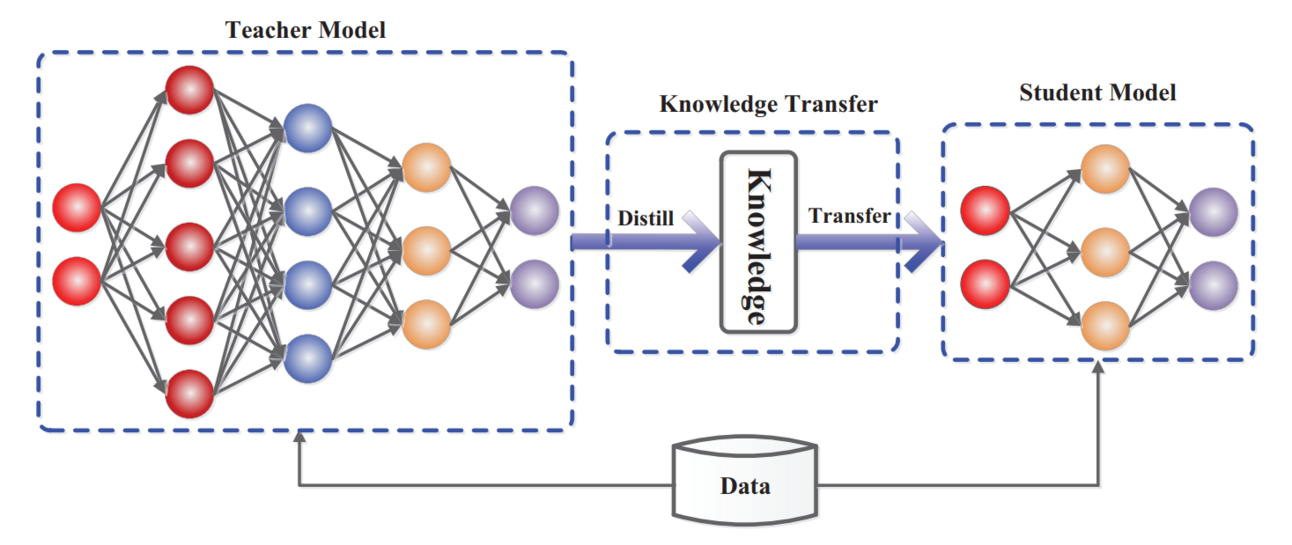
\includegraphics[width=0.8\textwidth]{knowledge_distillation.png}
    \captionof{figure}{Quy trình Chưng cất Tri thức. Mô hình trò học đồng thời từ nhãn cứng của dữ liệu và nhãn mềm (được tạo ra bởi mô hình thầy với nhiệt độ T).}
    \label{fig:knowledge_distillation}
\end{center}

Các mô hình như DistilBERT đã sử dụng kỹ thuật này để tạo ra một phiên bản BERT nhỏ hơn 40% và nhanh hơn 60% trong khi vẫn giữ lại 97% hiệu năng.

\subsection{Lượng tử hóa (Quantization)}
\label{ssec:quantization}

\subsubsection{Trực giác cốt lõi: Giảm độ chính xác của Số}
Lượng tử hóa là quá trình giảm số lượng bit được sử dụng để biểu diễn một con số. Trong học sâu, các trọng số và giá trị kích hoạt của mô hình thường được lưu trữ dưới dạng số thực dấu phẩy động 32-bit (FP32) hoặc 16-bit (FP16). Lượng tử hóa sẽ ánh xạ các giá trị này sang các định dạng có độ chính xác thấp hơn, ví dụ như số nguyên 8-bit (INT8) hoặc thậm chí 4-bit.

\begin{tcolorbox}[
    title=Triết lý của Lượng tử hóa,
    colback=blue!5!white, colframe=blue!75!black, fonttitle=\bfseries
]
"Chúng ta có thực sự cần đến 32 bit độ chính xác để lưu trữ mỗi trọng số không? Liệu việc làm tròn các trọng số thành một tập hợp các giá trị rời rạc, có độ chính xác thấp hơn có làm ảnh hưởng nhiều đến hiệu năng cuối cùng không?"
\end{tcolorbox}
Câu trả lời, một cách đáng ngạc nhiên, thường là "không nhiều". Các mạng nơ-ron sâu có một sự dư thừa (redundancy) nhất định và có khả năng chống chịu khá tốt với nhiễu và sự mất mát độ chính xác.

\subsubsection{Các phương pháp Lượng tử hóa}
\paragraph{Post-Training Quantization (PTQ) - Lượng tử hóa sau Huấn luyện}
Đây là phương pháp đơn giản nhất.
\begin{enumerate}
    \item Lấy một mô hình đã được huấn luyện đầy đủ.
    \item Chuyển đổi các trọng số của nó từ FP32/FP16 sang INT8. Quá trình này bao gồm việc tìm ra một "tỷ lệ" (scale) và một "điểm không" (zero-point) để ánh xạ khoảng giá trị thực sang khoảng giá trị nguyên 8-bit.
    \item Thường yêu cầu một bộ dữ liệu hiệu chỉnh nhỏ (calibration dataset) để tìm ra các tham số ánh xạ tối ưu.
\end{enumerate}
PTQ rất nhanh để thực hiện nhưng có thể gây ra sụt giảm độ chính xác đáng kể.

\paragraph{Quantization-Aware Training (QAT) - Huấn luyện Nhận biết Lượng tử hóa}
Đây là phương pháp phức tạp nhưng cho kết quả tốt hơn.
\begin{enumerate}
    \item Trong quá trình fine-tuning (hoặc huấn luyện từ đầu), mô hình sẽ \textbf{mô phỏng (simulate)} ảnh hưởng của việc lượng tử hóa.
    \item Tức là, trong quá trình truyền thẳng, các trọng số sẽ được "làm tròn" (quantized) về định dạng có độ chính xác thấp, nhưng trong quá trình truyền ngược, gradient vẫn được tính toán và cập nhật trên các trọng số có độ chính xác đầy đủ.
    \item Điều này cho phép mô hình học cách "thích ứng" với sự mất mát độ chính xác sẽ xảy ra sau khi lượng tử hóa, giúp giảm thiểu sụt giảm hiệu năng.
\end{enumerate}

Lợi ích của Lượng tử hóa là rất rõ ràng: giảm kích thước mô hình (INT8 nhỏ hơn FP32 4 lần) và tăng tốc độ suy luận (các phép toán trên số nguyên nhanh hơn nhiều so với số thực trên hầu hết các phần cứng). Chúng ta đã thấy một ứng dụng của nó trong QLoRA (mục \ref{ssec:qlora}).

\subsection{Cắt tỉa (Pruning)}
\label{ssec:pruning}

\subsubsection{Trực giác cốt lõi: Loại bỏ các Kết nối Thừa}
Các mạng nơ-ron lớn thường được "tham số hóa quá mức" (over-parameterized), nghĩa là chúng có nhiều trọng số và nơ-ron hơn mức cần thiết. Cắt tỉa là quá trình xác định và loại bỏ các trọng số hoặc các nơ-ron "ít quan trọng" nhất trong mạng.

\begin{tcolorbox}[
    title=Triết lý của Cắt tỉa,
    colback=red!5!white, colframe=red!75!black, fonttitle=\bfseries
]
"Một mạng nơ-ron giống như một cái cây. Sau khi nó phát triển, chúng ta có thể cắt tỉa đi những cành lá không cần thiết mà không làm ảnh hưởng đến sức sống và khả năng ra quả của cây, thậm chí còn giúp cây khỏe mạnh hơn."
\end{tcolorbox}

\subsubsection{Các phương pháp Cắt tỉa}
\paragraph{Cắt tỉa theo Độ lớn (Magnitude Pruning)}
Đây là phương pháp phổ biến nhất.
\begin{itemize}
    \item \textbf{Giả định:} Các trọng số có giá trị tuyệt đối gần bằng 0 là ít quan trọng nhất.
    \item \textbf{Quy trình:}
        \begin{enumerate}
            \item Huấn luyện một mô hình dày đặc đến khi hội tụ.
            \item Xóa (đặt bằng 0) tất cả các trọng số có giá trị tuyệt đối nhỏ hơn một ngưỡng nhất định. Điều này tạo ra một ma trận trọng số "thưa thớt" (sparse).
            \item (Tùy chọn nhưng quan trọng) Fine-tune lại mô hình thưa thớt này trong một vài epoch để cho phép các trọng số còn lại "bù đắp" cho các trọng số đã bị xóa.
        \end{enumerate}
\end{itemize}

\paragraph{Cắt tỉa có Cấu trúc vs. Không có Cấu trúc (Structured vs. Unstructured Pruning)}
\begin{itemize}
    \item \textbf{Không có cấu trúc:} Xóa các trọng số riêng lẻ ở bất kỳ đâu trong ma trận. Điều này tạo ra các ma trận thưa thớt, có thể giảm đáng kể số lượng tham số nhưng không phải lúc nào cũng tăng tốc độ trên phần cứng thông thường (như GPU) vốn được tối ưu cho các phép toán ma trận dày đặc.
    \item \textbf{Có cấu trúc:} Xóa toàn bộ các cấu trúc lớn hơn, ví dụ như xóa toàn bộ một nơ-ron (một cột trong ma trận trọng số) hoặc toàn bộ một bộ lọc trong CNN. Phương pháp này có thể không giảm được nhiều tham số bằng, nhưng kết quả là một mô hình nhỏ hơn, dày đặc hơn, có thể chạy nhanh hơn trên phần cứng hiện có mà không cần các thư viện đặc biệt.
\end{itemize}

\begin{center}
    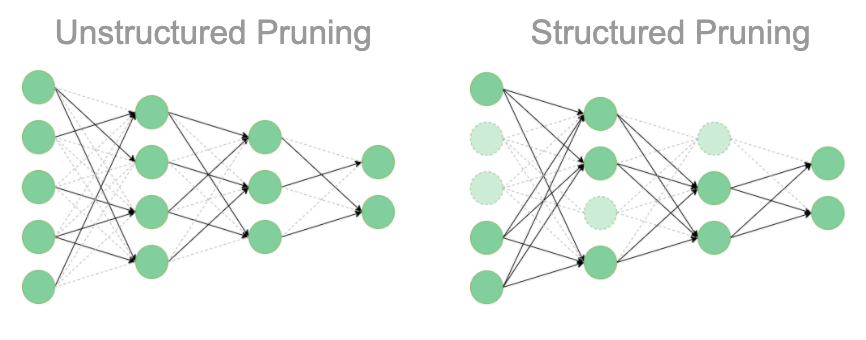
\includegraphics[width=1.0\textwidth]{pruning_types.png}
    \captionof{figure}{So sánh Cắt tỉa Không có Cấu trúc (xóa các trọng số riêng lẻ, tạo ma trận thưa thớt) và Cắt tỉa Có Cấu trúc (xóa toàn bộ cột/nơ-ron, tạo ma trận nhỏ hơn).}
    \label{fig:pruning_types}
\end{center}

Các kỹ thuật tối ưu hóa này thường được sử dụng kết hợp với nhau (ví dụ, một mô hình được chưng cất, sau đó được cắt tỉa và cuối cùng được lượng tử hóa) để đạt được sự cân bằng tốt nhất giữa kích thước, tốc độ và độ chính xác.